\begin{frame}
\frametitle{Erros e Avisos}
\framesubtitle{}
\centering
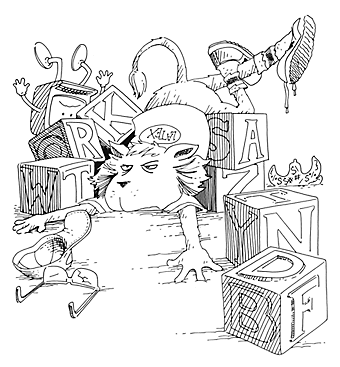
\includegraphics[width=0.5\linewidth]{figures/lion03.png}
\end{frame}


\begin{frame}[fragile]
\frametitle{Erros e Avisos}
\framesubtitle{Errar é inevitável!}

\begin{itemize}
\item achar/reconhecer os seus erros costuma ser a tarefa mais difícil
\item não entre em pânico
\item muitas vezes o erro não está no local onde foi detectado
\end{itemize}

\begin{verbatim}
! Undefined control sequence.

! Too many }'s.

! Missing $ inserted

Runaway argument?

Overfull \hbox 

! LaTeX Error: File `paralisy.sty' not found.
\end{verbatim}
\end{frame}

\begin{frame}[fragile]
\frametitle{Erros e Avisos}
\framesubtitle{Não deixe que os erros virem monstros}
Dica:
\begin{itemize}
\item cada passo de uma vez
\item mantenha um controle de versão (ou backup)
\end{itemize}
\end{frame}


\begin{frame}[fragile]
\frametitle{Coding is like cooking}
\framesubtitle{}
\begin{figure}[h!]
  \centering
  \label{fig:cooking}
  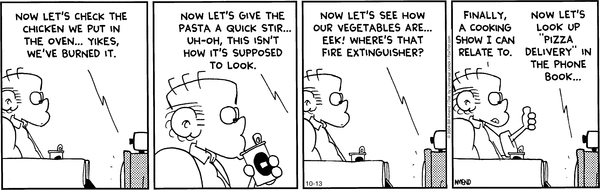
\includegraphics[width=0.8\textwidth]{figures/cooking.png}
  \caption{Coding and Cooking (Bill Amend).}
\end{figure}

\end{frame}


